\section{MLCommons Medical AI}
{{\footnotesize
\begin{description}[labelwidth=5em, labelsep=1em, leftmargin=*, align=left, itemsep=0.3em, parsep=0em]
  \item[date:] 2023-07-17
  \item[last\_updated:] 2023-07
  \item[expired:] unkown
  \item[valid:] yes
  \item[url:] \href{https://github.com/mlcommons/medical}{https://github.com/mlcommons/medical}
  \item[domain:] Healthcare; Medical AI
  \item[focus:] Federated benchmarking and evaluation of medical AI models across diverse real-world clinical data
  \item[keywords:]
    - medical AI
    - federated evaluation
    - privacy-preserving
    - fairness
    - healthcare benchmarks
  \item[task\_types:]
    - Federated evaluation
    - Model validation
  \item[ai\_capability\_measured:]
    - Clinical accuracy
    - fairness
    - generalizability
    - privacy compliance
  \item[metrics:]
    - ROC AUC
    - Accuracy
    - Fairness metrics
  \item[models:]
    - MedPerf-validated CNNs
    - GaNDLF workflows
  \item[ml\_motif:]
    - Multiple
  \item[type:] Platform
  \item[ml\_task:] NA
  \item[notes:] Open-source platform under Apache‑2.0; used across 20+ institutions and hospitals :contentReference[oaicite:2]\{index=2\}.
  \item[contact.name:] Alex Karargyris (MLCommons Medical AI)
  \item[contact.email:] unkown
  \item[dataset.name:] Multi-institutional clinical datasets
  \item[dataset.url:] \href{radiology}{radiology}
  \item[results.name:] ChatGPT LLM
  \item[results.url:] \href{unkown}{unkown}
  \item[fair.reproducible:] Yes
  \item[fair.benchmark\_ready:] Yes
  \item[ratings.software.rating:] 0
  \item[ratings.software.reason:] Not analyzed.
  \item[ratings.specification.rating:] 9.0
  \item[ratings.specification.reason:] Diverse scientific tasks (earthquake, CFD, microscopy) with detailed problem statements and goals; system constraints not uniformly applied.
  \item[ratings.dataset.rating:] 9.0
  \item[ratings.dataset.reason:] Domain-specific datasets (e.g., microscopy, climate); mostly public and structured, but FAIR annotations are not always explicit.
  \item[ratings.metrics.rating:] 9.0
  \item[ratings.metrics.reason:] Task-specific metrics (MAE, speedup, accuracy) are clear and reproducible.
  \item[ratings.reference\_solution.rating:] 9.0
  \item[ratings.reference\_solution.reason:] Reference models (CNN, GNN, Transformer) provided with training/evaluation pipelines.
  \item[ratings.documentation.rating:] 9.0
  \item[ratings.documentation.reason:] Well-documented, open-sourced, and maintained with examples; strong community support and reproducibility focus.
  \item[id:] mlcommons\_medical\_ai
  \item[Citations:] \cite{karargyris2023federated}
  \item[Ratings:]
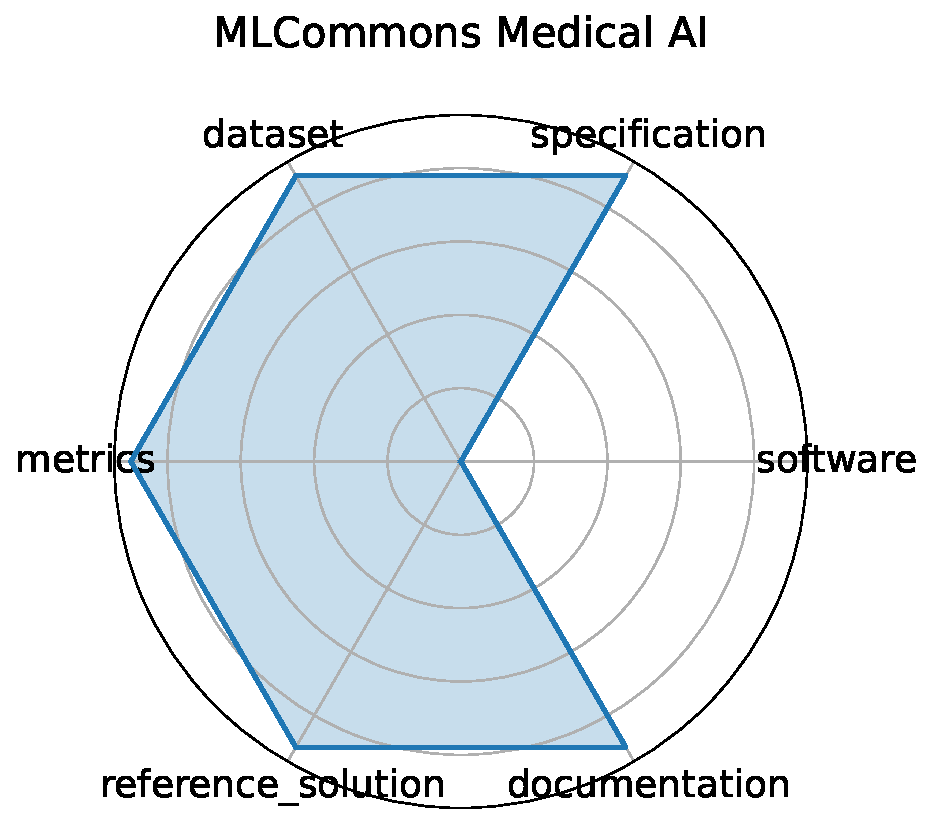
\includegraphics[width=0.2\textwidth]{mlcommons_medical_ai_radar.pdf}
\end{description}
}}
\clearpage